\quad Para implementar el estimador seg\'un el paper de Piatetsky-Shapiro, nos basamos en la implementaci\'on que estima con el menor error para el peor caso. Hay otra implementaci\'on que se basa en los casos  de error promedio m\'as chico.

\quad En su paper, Piatetsky-Shapiro determinan casos donde puede caer un valor en alg\'un tipo de step. Siendo X el valor buscado ya sea por igualdad o por mayor, los casos y sus errores son los siguientes: \\

\begin{itemize}
\item \textbf{A) X est\'a entre steps:} \quad $ \frac{2}{3} * S$ \\

\item \textbf{B1) X es igual al valor de un step I pero I no es el primer step ni el \'ultimo:} \quad $ \frac{1}{S} $ \\

\item \textbf{B2) X es igual al valor de varios steps pero no incluye al primer step ni al \'ultimo:} \quad $ \frac{1}{S} $ \\

\item \textbf{C) X es igual al valor de uno o varios steps, pudiendo incluir al primer o \'ultimo step:} \quad $ \frac{1}{S} $ \\

\item \textbf{D) X est\'a afuera del rango de posible valores:} \quad $ 0 $ \\
\end{itemize}

\textbf{Aclaraci\'on:} \quad En el paper no figura cota de error para el caso C, por lo que asumimos que es igual a los anteriores, ya que la diferencia est\'a en que puede incluir al primer step o al \'ultimo. \\

\quad A continuaci\'on presentamos el gr\'afico derivado de la figura 14: \\

\begin{figure}[H]
	  \begin{center}
	    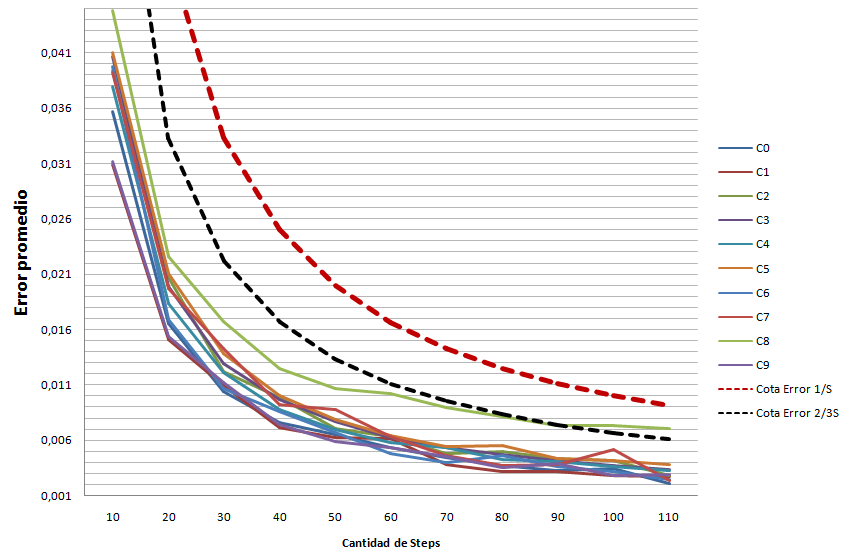
\includegraphics[scale=.70]{imagenes/StepsCotasDeError.png}
	    \caption{Error del estimador de pasos distribuidos sobre todas las columnas y las cotas de error} 
	    \label{fig:(StepsErrorCota}
	  \end{center}
	\end{figure}
	
\quad Como podemos ver, todas salvo la columna C8, cumplen con las cotas. Se observa, que a medida que var\'ia la cantidad de steps, no cambia considerablemente la diferencia entre el error y las cotas. \\

\quad En cuanto a la columna C8, analizando su distribuci\'on y el algoritmo de pasos distribuidos pudimos comprobar que hay un problema con el algoritmo del cual no se habla en el paper.

\quad El rango de la columna C8 es de 0 a 41. El algoritmo de pasos distribuidos determina el valor de un step I como el elemento que se encuentran en la posici\'on (1 + I*N), donde $ N = \frac{T-1}{S} $ y S es el valor del par\'ametros que simboliza la cantidad total deseada de steps y T la cantidad total de tuplas en la tabla. Debido a esto, cuando la cantidad de steps es mayor a la cantidad de elementos por steps se produce un error. Debido al rango de las dem\'as columnas, nuestros testeos los realizamos con un valor alto de cantidad de steps. Alto comparando con el espectro de la columna C8. Adjudicamos a eso el por qu\'e a partir de cierto punto el error rompe la cota para esa columna. 